
Para que o um veículo aéreo não tripulado funcione de forma completa, é necessário definir um sistema de fornecimento de energia eficiente, para que o mesmo consiga suprir todas as necessidades dos sistemas que terão funções de controle e comando.

\subsubsection{Bateria}

Uma bateria é um dispositivo capaz de armazenar energia química e transformá-la em energia elétrica. A bateria é entendida geralmente como algo que possui duas ou mais células elétricas individuais, e existem dois tipos básicos de células: primária e secundária \cite{gibbs}. As primárias, identificadas como células normais, não são recarregáveis e devem ser descartadas quando esgotadas. Já as secundárias, são recarregáveis, como a bateria do tipo polímero de lítio, que foi a escolhida para atuar neste projeto, e será apresentada posteriormente. 

Para determinar a escolha da bateria utilizada em qualquer projeto, é importante fazer a análise  da energia armazenada na bateria e a variação de descarga ao ser utilizada, e para calcular a energia armazenada, deve-se conhecer a tensão (V) e sua capacidade de descarga de corrente no tempo (Ah), utilizando a equação a seguir: \cite{peixoto}

Além disso, deve-se também conhecer a densidade de energia (relação entre quantidade de energia por unidade de massa ou Volume), Resistência interna, voltagem, peso, viabilidade econômica e disponibilidade no mercado.

$Energia(Wh)= Tensão(V)*Capacidade(Ah)$

\subsubsection{Bateria de polímeros de Lítio (Li-Polymer)}

Baterias de polímeros de Lítio (LiPo) são aquelas que contem seus eletrólitos retidos em um polímero sólido, 
composta por várias células secundárias finas idênticas ligadas em paralelo, o que aumenta sua capacidade de 
descarga, sendo essencial que ela opere em uma faixa entre sua voltagem, não excedendo nem diminuindo muito, para perfeito funcionamento. \cite{gibbs}

As células de lítio-polímero são feitas de três componentes principais: um catodo (placa positiva), um anodo 
(placa negativa) e um separador. O catodo e o anodo são feitos principalmente de lítio, já o separador é feito 
de folhas rígidas de polímero banhadas em eletrólito. \cite{gibbs}

São flexíveis e oferecem leveza, já que não se faz necessário uma camada metálica externa como as baterias de 
Lítio-Íon, e podem ser facilmente moldadas para diversas aplicações. Também possuem uma resistência interna 
baixa que se adequa bem as altas taxas de descargas. \cite{costa}. Usada comercialmente desde 1999 as baterias 
de polímeros de Lítio possuem densidade de energia em torno de 100 e 130 Wh/kg, ou seja, quantidade de energia 
por volume relativamente alta, muito parecida com as baterias de Lítio-Íon. Com isso o fator mais importante para
análise é a tolerância para a sobrecarga, nas baterias de Lítio-polímero essa tolerância é maior, evitando um 
excesso de energia concentrado na bateria que ocasionaria a perda de rendimento ou até a perda total da bateria.
\cite{costa}

\subsubsubsection{Características bateria LiPo 6s}

O funcionamento básico da célula de bateria do tipo LiPo consiste em eletrólitos de sais de lítio retidos
em um polímero sólido com óxido de polietileno e o poliacrilonitrilo ao invés de solventes tornando-as
adaptáveis a diferentes formatos e permitindo altas taxas de descarga. A carga elétrica de uma bateria
corresponde a quantidade de carga, corrente, que pode ser fornecida por uma hora. 
A taxa de descarga corresponde ao quanto essa carga pode ser dissipada no mesmo intervalo de tempo. \cite{gibbs}

Suas principais vantagens são: peso reduzido em comparação com as demais e fornecimento de altas correntes 
\cite{pinto}. Apesar de suas vantagens e de ser utilizada como um combustível e não como bateria,
as baterias de LiPo estão propensas a sobrecarga durante o processo de carga devido a diversos fatores, 
o que pode ocasionar combustão. Com isso, é necessária a utilização de carregadores adequados, ajuste correto 
de taxa de carga, utilização de balanceador de células evitando que a carga seja aplicada diretamente aos 
terminais principais do pack sem controle de voltagem, além de evitar o procedimento de carga ao identificar 
que as células do pack estão danificadas. \cite{gibbs}

\subsubsubsection{Recarga}

A carga de uma bateria é explicada de forma simples por um fenômeno químico-físico que está envolvido com a eletrólise. \cite{gibbs}

Entretanto, essa simplicidade não deve ser subestimada, pois existem detalhes nesse tipo de bateria (Lipo 6s) que precisam ser levados em consideração dependendo da sua forma de uso.

Para o recarregamento da bateria que alimentará o VANT, será utilizada uma plataforma de recarga que funcionará diretamente ligada à  central de energia da estação de controle e fornecerá a energia necessária para o recarregamento da bateria quando o VANT necessitar.

A plataforma funcionará a partir de cabos específicos que estarão ligados a central energética da estação de controle. Assim, toda vez que o VANT retornar para a central alguma pessoa capacitada conectará o mesmo à plataforma de recarga. Ao aviso de recarga da bateria do VANT, a pessoa encarregada pela central desconectará os cabos.

A bateria de polímero de Lítio caso esteja acima da temperatura normal na hora da recarga, deve ser levada para um local afastado e ventilado, para que sua temperatura normalize.A maioria dos acidentes com baterias ocorrem durante a recarga. A bateria de lítio polimerizado em comparação com as outras tem um baixo risco de acidente nesse requisito. \cite{gibbs}

As baterias de Lítio Polimerizado tem dois requerimentos em relação as suas células, primeiramente a carga deve ser limitada a um valor seguro e em segundo lugar, a voltagem da célula não deve nunca ultrapassar 4.20 Vpc (Volts por célula). \cite{gibbs}

O carregador Li-PO é um dispositivo limitador de tensão que é semelhante ao sistema de chumbo-ácido. A diferença está em uma tensão mais elevada por célula, tolerância de tensão mais apertado e a ausência de carga de flutuação em plena carga.

As baterias de polímero de Lítio não podem ser carregadas por qualquer tipo de carregador, portanto, o escolhido para atuar no sistema de recarga do EmerVant foi o carregador iMax B6 (figura \ref{fig:carregador1}), se adequa de uma forma que carrega e balanceia adequadamente vários tipos de bateria de lítio, tais como a utilizada neste projeto (LiPo 6s), Li-íon e a série de bateria LiFe.


 \begin{figure}[h!]
    \centering
	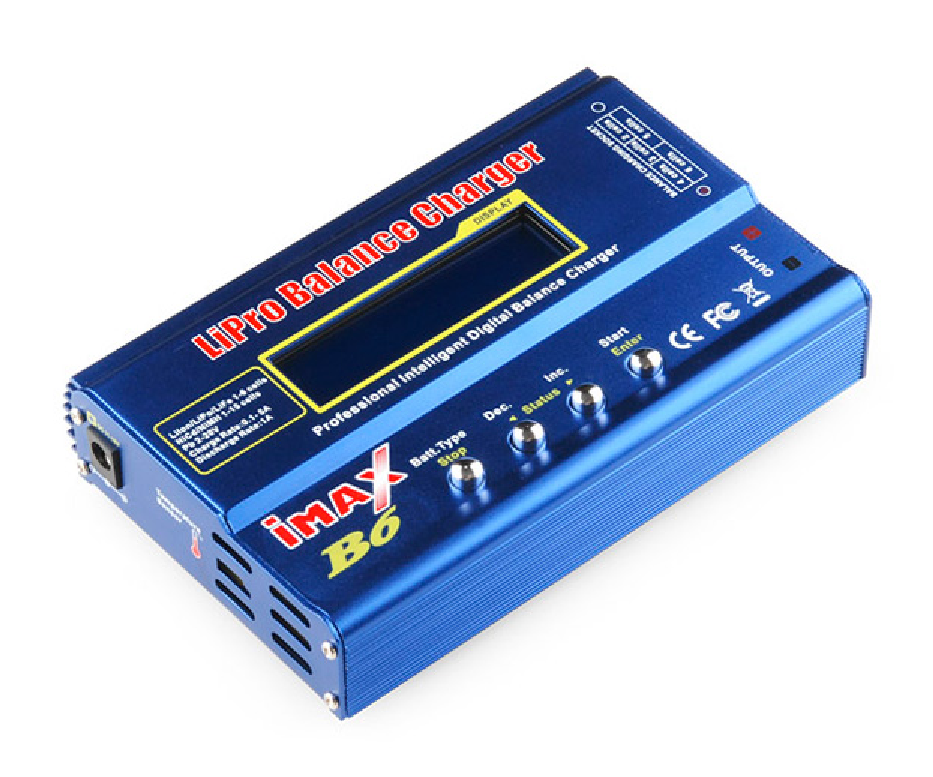
\includegraphics[keepaspectratio=true,scale=0.4]{figuras/carregador1.eps}
    \caption{Carregador iMax B6. Fonte: \cite{carregador1}}
    \label{fig:carregador1}
\end{figure}


Segundo o manual do usuário iMax B6 \cite{ibmax}, independente de qual seja a bateria de lítio usada, não será necessário se conectar a um balanceador externo para efetuar a carga de balanceamento, pois o mesmo emprega um balanceador de tensão de célula individual. Além disso, o B6 monitora e balanceia individualmente cada célula da bateria, onde apresenta uma mensagem de erro e é automaticamente interrompido caso apresente uma tensão anormal de qualquer célula individual. 

A figura a seguir mostra o menu do B6, que possui uma interface fácil de se interpretar, onde indica o carregamento e os ciclos em um processo simples, podendo ser feito de maneira rápida e precisa. O carregador não vem com a fonte de alimentação, porém contém um conector de entrada de CC que possui um \textit{plug} com garras tipo jacaré.

 \begin{figure}[h!]
    \centering
	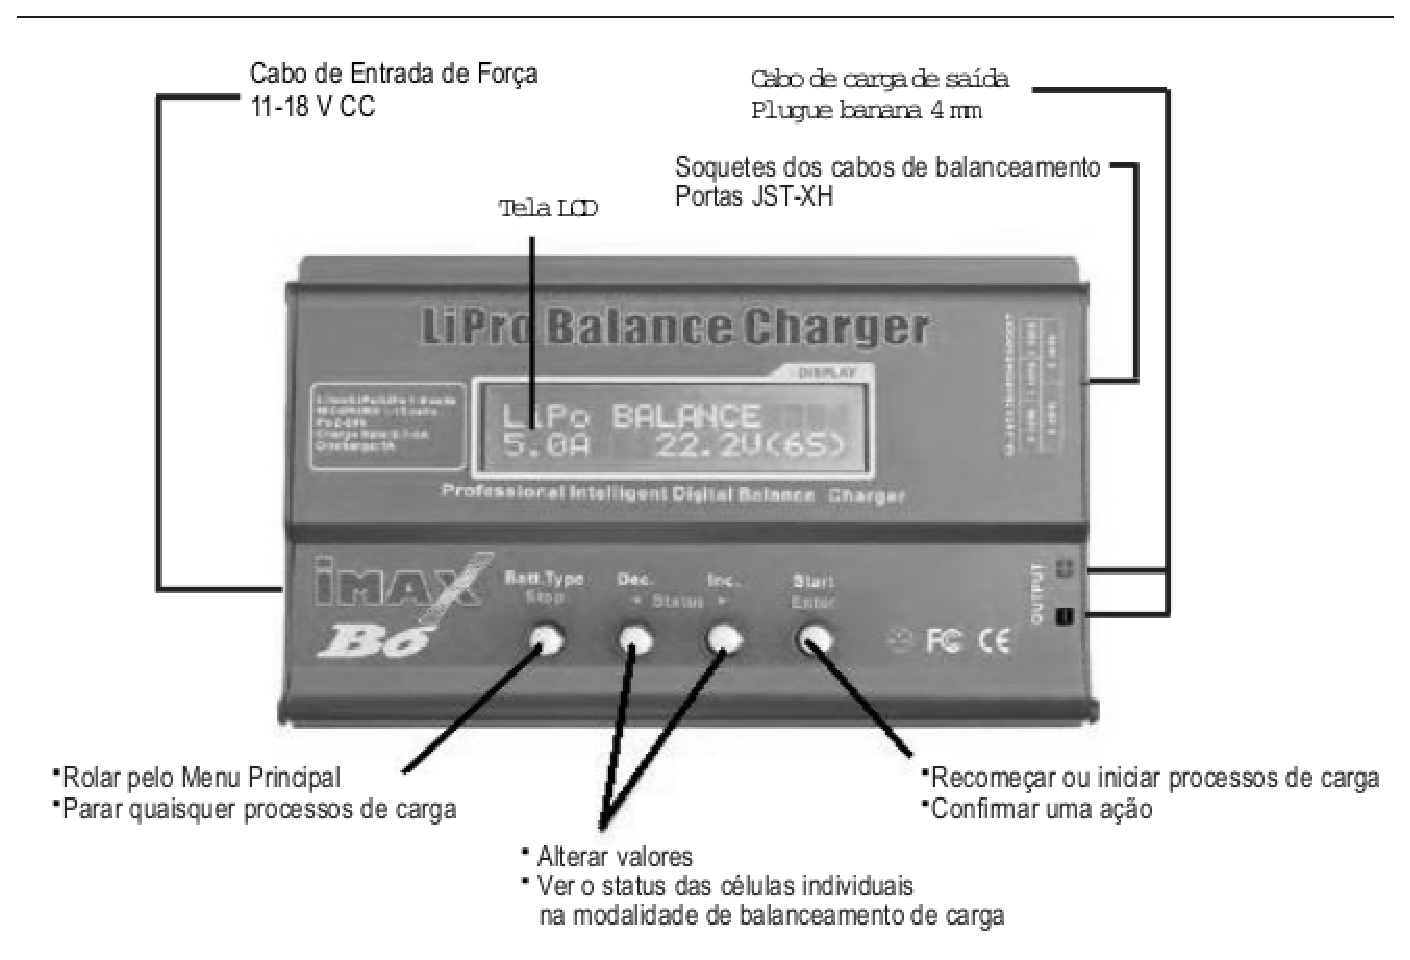
\includegraphics[keepaspectratio=true,scale=0.5]{figuras/manual.eps}
    \caption{Menu do iMax B6. Fonte: \cite{ibmax}}
\end{figure}


\subsubsubsection{Análise de Custos}

Considerando os requisitos estipulados  no escopo do projeto foram levantadas discussões e pesquisas que culminaram na escolha da tecnologia lítio polímero (LiPO) para utilização na parte da alimentação energética do VANT. Essa tecnologia se sobressaiu em relação a todas outras estudadas por baterias que apresentam baixo peso, alta tensão, além de sua capacidade de fornecer elevadas correntes ao circuito e já ser uma tecnologia amplamente utilizada no meio aeroespacial.

Durante a escolha da bateria foram analisadas várias empresas ao redor de todo o mundo, sendo elas:

\begin{itemize}
 
\item Gens Tattu (Americana)

\item Foxtech (Chinesa)

\item Max Amps (Americana)

\item Robokits (Indiana)

\item Dronera (Norueguesa)

\item Honcell (Chinesa)

\end{itemize}


A empresa fornecedora foi escolhida com base em diversos aspectos, os quais foram: impostos relativos a importação, facilidade de contato com os fabricantes, renome internacional da empresa, densidade energética da bateria além do custo da bateria.

A  Tattu foi a empresa escolhida como fornecedora da bateria.  Dentre os fatores que mais pesaram na escolha foram a proximidade em relação ao Brasil, a facilidade de comunicação com o fabricante e também a qualidade da bateria. Foi observado que mesmo nas diferentes áreas ao redor do mundo as baterias não apresentam uma grande variação em relação ao custo, o que também favoreceu a empresa americana visto que as taxas de importação são relativamente inferiores, sendo que as únicas baterias relativamente mais baratas eram aquelas com um peso bastante superior às outras.

As especificações da bateria escolhida levam como base a potência necessária de vôo do VANT, que por sua vez está relacionada ao tempo de vôo e também ao seu peso.  Serão necessárias apenas uma bateria com capacidade de 16000 mAh, o que somaria 400 dólares ao custo do projeto, cerca de 1200 reais de acordo com as cotações atuais. Abaixo segue todas as especificações da bateria escolhida, assim como uma tabela de comparação entre as outras baterias encontradas no mercado. 
As informações contidas na tabela foram retiradas dos sites de vendas dos fabricantes.
 \begin{figure}[h!]
    \centering
	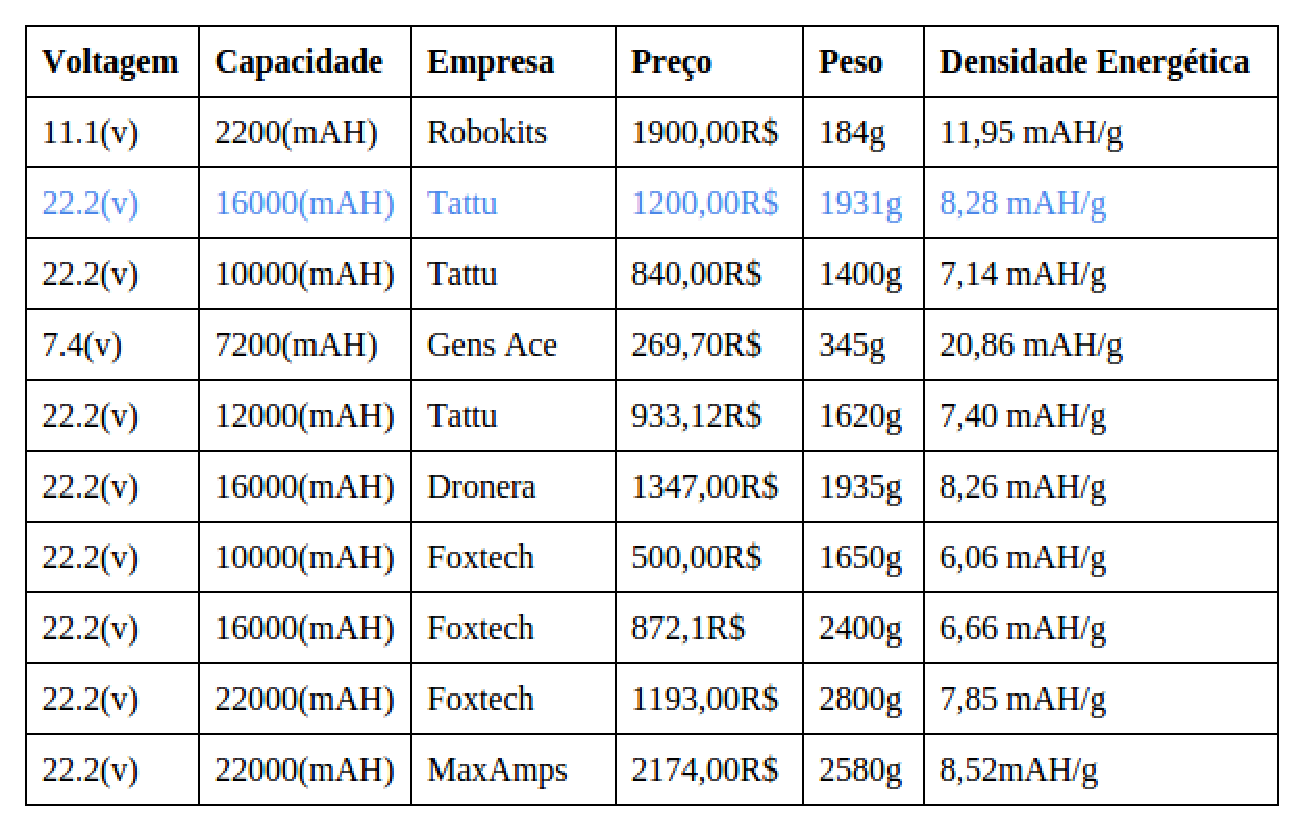
\includegraphics[keepaspectratio=true,scale=0.7]{figuras/comparacaobaterias.eps}
    \caption{Tabela comparativa entre baterias}
\end{figure}

\nocite{bateria1}
\nocite{bateria2}
\nocite{bateria3}
\nocite{bateria4}
\nocite{bateria5}
\nocite{bateria6}
\nocite{bateria7}
\nocite{bateria8}
\nocite{bateria9}
\nocite{bateria10}


\subsubsection{Conceitos e características para obter a autonomia do EmerVant}

Os conceitos foram baseados em \cite{charlesa}, \cite{charlesb} e \cite{gibbs}.

\textbf{-Densidade de energia} (wh/kg) - é a relação entre a quantidade de energia contida em um dado sistema ou região do espaço e o volume ou massa, dependendo do contexto, deste sistema/região.

	Densidade de energia EmerVant: $\frac{355wh}{1932kg} =  183,85 wh/kg$

\textbf{-Capacidade} (amp-hora ou mA-h) -  O mA-h é a abreviação usada como padrão para o \textit{miliampere}-hora, uma subunidade de medida (advinda do \textit{ampere}-hora, ou apenas Ah) utilizada para reconhecer a transferência de carga elétrica através de uma corrente estável de um \textit{ampere} no período de uma hora.

	Capacidade EmerVant: $16.000mA-h$

\textbf{-Tensão elétrica} (V) ou diferença de potencial (DDP) - é a diferença de potencial elétrico entre dois pontos ou a diferença em energia elétrica potencial por unidade de carga elétrica entre dois pontos. Sua unidade de medida é o \textit{volt}.
	
	Tensão do EmerVant: $22.2 V$

\textbf{-Resistência interna} (W) - é a capacidade de um corpo qualquer se opor à passagem de corrente elétrica mesmo quando existe uma diferença de potencial aplicada. A presença da resistência interna da bateria limita a sua voltagem de acordo com a corrente que passa pelo circuito.

	Resistência interna do EmerVant: $1\Omega$

\textbf{-Taxa de descarga} (mA) - é a corrente eléctrica aplicada a uma bateria com o objectivo de restaurar a sua capacidade energética. Esta taxa encontra-se por regra estandardizada relativamente à capacidade total de armazenamento da bateria e a um dado período de tempo.

\textbf{-Vida útil} - é o período em que a bateria funciona em modo eficiente. O tempo que a bateria dura entre cargas, assim como a vida útil da bateria, irá variar dependendo de vários fatores. São resumidos geralmente em seus ciclos de recarga.
	
	Vida útil do EmerVant: $500-1000 vezes$

\textbf{-Autonomia} - é a duração em horas que funcionará a bateria sem recarga. \cite{esteban}. Onde:

E - Energia total armazenada na bateria

P - Potência de saída

T - Tempo

TT - Empuxo total

Logo,

$ET= 22.2 V * 16MAh= 355Wh$

$Densidade = \frac{ET}{P}$

$Densidade = 183.85$

$ET= \frac{TT}{TE*1H}$

$ET = \frac{7810}{7.69*1H} = 1015.60 Wh$

Portanto, a autonomia do VANT será determinada por:

$Autonomia = \frac{355WH}{1015.60Wh}$

$Autonomia = 0.3495 horas$, $aproximadamente$ $20$ $minutos$
